\documentclass[12pt]{article}
\usepackage[utf8]{inputenc}
\usepackage[a4paper,margin=1in]{geometry}
\usepackage{amsmath,amssymb}
\usepackage{enumitem}
\usepackage{parskip}
\usepackage{xcolor}
\usepackage{fancyhdr}
\usepackage{tikz}
\usepackage{graphicx}
\usepackage{eso-pic}
\usepackage{titlesec}

\graphicspath{{../}}

\definecolor{kcpc-bg}{RGB}{250,250,250}
\definecolor{kcpc-text}{RGB}{20,20,20}
\definecolor{kcpc-muted}{RGB}{90,90,90}
\definecolor{kcpc-red}{RGB}{176,0,0}

\newcommand{\kcpcwordmark}{\raisebox{-0.15\height}{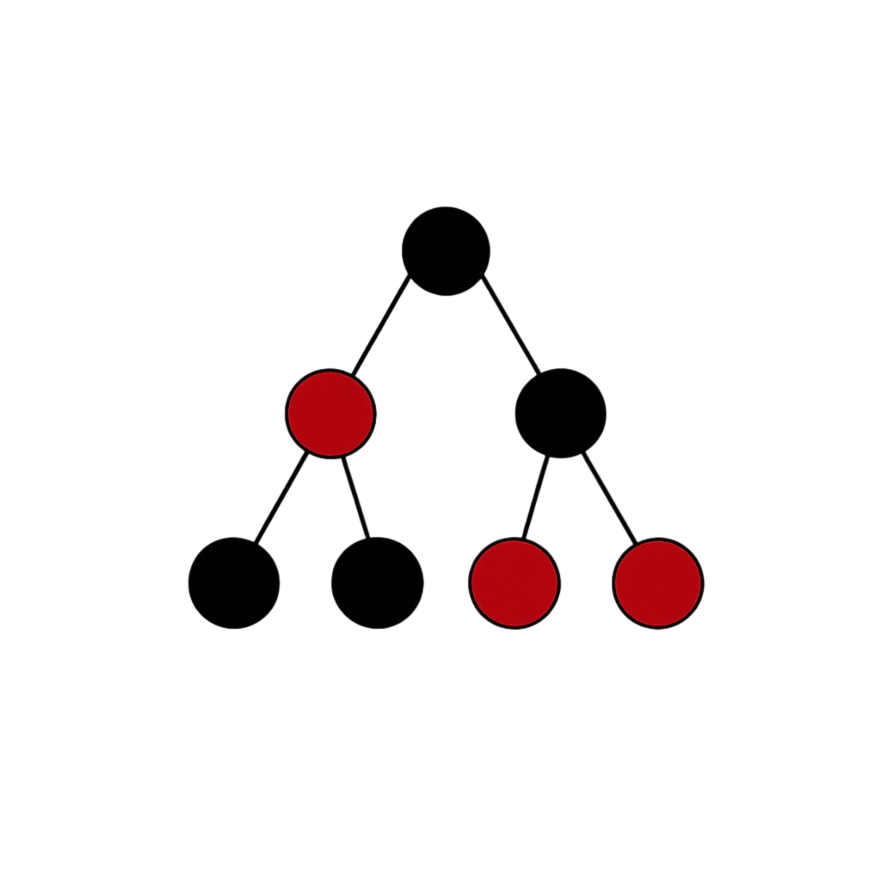
\includegraphics[height=0.55cm]{kcpc-logo.png}}}

\pagestyle{fancy}
\fancyhf{}
\lhead{\textcolor{kcpc-text}{\small\bfseries Solutions}}
\rhead{\textcolor{kcpc-muted}{\small Week 1}}
\cfoot{\textcolor{kcpc-muted}{\small KCPC}}
\renewcommand{\headrulewidth}{0.4pt}
\renewcommand{\headrule}{\hbox
to\headwidth{\color{kcpc-red}\leaders\hrule height \headrulewidth\hfill}}
\renewcommand{\footrulewidth}{0pt}
\setlength{\headheight}{28pt}

\AddToShipoutPictureBG{%
    \begin{tikzpicture}[remember picture,overlay]
        \node[opacity=0.035, at=(current page.center)]
        {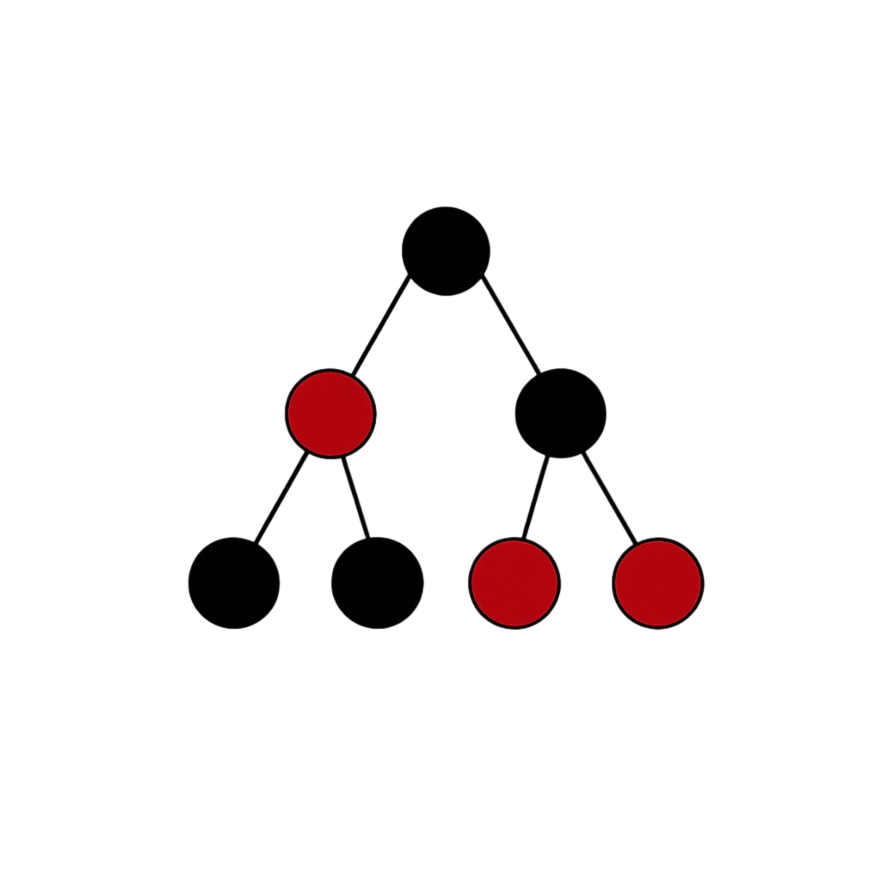
\includegraphics[width=0.38\paperwidth]{kcpc-logo.png}};
    \end{tikzpicture}%
}

\titleformat{\section}{\large\bfseries\color{kcpc-red}}{\thesection}{1em}{}

\setlist[itemize]{noitemsep, topsep=4pt}
\setlist[enumerate]{topsep=4pt}

\newcommand{\insight}[1]{\par\medskip\noindent\textbf{Key insight:} #1}

\title{KCPC Week 1 Solutions}
\author{}
\date{}

\begin{document}
\maketitle
\thispagestyle{fancy}

\section{Logic}

\subsection*{Basic -- Same Birthday Month}
There are only 12 months. If 13 students are placed into 12
month-boxes by birth month, the pigeonhole principle forces at least
one box to contain at least two students.

\subsection*{Easy -- Glove Selection}
For one matching pair, the adversarial draw is all gloves of the same
hand: $5+3+2=10$ gloves. The next glove guarantees a pair, so the answer is 11.

For one matching pair of each colour, the worst case is all 10 black
gloves, all 6 brown gloves, and 2 grey gloves of the same hand. The
next grey glove completes the final pair, so the answer is 19.

\subsection*{Medium -- Three People: Knights, Knaves, and Spies}
Let the types be $K$ (Knight), $N$ (Knave), $S$ (Spy). Exactly one of
each exists. Alice says ``Bob is $N$''; Bob says ``Carol is $K$''; Carol
says ``Alice is $S$''.

Suppose Alice is $K$. Then Bob is $N$, so Bob lies. Bob says ``Carol is
$K$'', so Carol is not $K$. Carol must be $S$. Then Alice is $K$, Bob
is $N$, Carol is $S$ -- consistent. Carol says ``Alice is $S$'', which
is false; as Spy she may lie. This works.

Suppose Bob is $K$. Then Carol is $K$, contradiction (two Knights).

Suppose Carol is $K$. Then Alice is $S$, so Alice is not $K$. Bob must
be $K$ (only one $K$), but then Carol is $K$ -- contradiction.

The only consistent assignment: Alice = Knight, Bob = Knave, Carol = Spy.
\insight{Test each possible assignment of the unique Knight; contradictions narrow it down.}

\subsection*{Hard -- Islander Statements}
Let $L$ be the number of liars. Statement $i$ is true exactly when
$L\ge i$. Therefore the true statements are precisely $1,2,\ldots,L$,
so there are $L$ truth-tellers and $10-L$ liars. But $L$ is the
number of liars, so $L=10-L$, hence $L=5$. Islanders 1 through 5 tell
the truth; islanders 6 through 10 lie.

\subsection*{Very Hard -- Counterfeit Coin}
One standard strategy is as follows. Label the coins $1$ to $12$.
First weigh $1,2,3,4$ against $5,6,7,8$.

If they balance, the counterfeit is among $9,10,11,12$. Weigh
$9,10,11$ against $1,2,3$. If this balances, coin 12 is counterfeit;
compare it with coin 1 to decide heavy/light. If it does not balance,
the odd coin is one of $9,10,11$ and its direction is known; weigh 9
against 10 to identify it.

If the first weighing is unbalanced, suppose $1,2,3,4$ are heavier
than $5,6,7,8$; the other case is symmetric. Then the counterfeit is
either heavy among $1,2,3,4$ or light among $5,6,7,8$. Weigh $1,2,5$
against $3,6,9$. If left is heavy, the counterfeit is heavy 1 or 2,
or light 6; weigh 1 against 2 to decide. If right is heavy, the
counterfeit is heavy 3 or light 5; weigh 3 against 9 to decide. If
balanced, the counterfeit is heavy 4, light 7, or light 8; weigh 7
against 8 to decide.

\section{Invariants}

\subsection*{Basic -- Jigsaw Assembly}
Each move reduces the number of sections by exactly 1. Starting with
500 sections and ending with 1 requires 499 moves.

\subsection*{Easy -- Odd Handshakes}
Sum the number of handshakes made by each person. This total equals
twice the number of handshakes, so it is even. The people with even
handshake counts contribute an even amount to the sum. Therefore the
people with odd handshake counts must also contribute an even amount.
A sum of odd numbers is even only when there are an even number of them.

\subsection*{Medium -- Chameleons}
Track the differences between colour counts modulo 3. A meeting
changes two colour counts by $-1$ and the third by $+2$, so
differences are unchanged modulo 3. Initially the differences include
$14-10=4\equiv1$, $15-14=1\equiv1$, and $15-10=5\equiv2\pmod3$. If
all colours became equal except one colour present, some relevant
difference would be $0\pmod3$. The invariant prevents this, so it is impossible.

\subsection*{Hard -- The MU Puzzle}
Track the number of \texttt{I}'s modulo 3. Initially it is 1. Rules 1
and 4 do not change it, Rule 2 doubles it, and Rule 3 subtracts 3.
Starting from a number not divisible by 3, these operations never
make it divisible by 3. The string \texttt{MU} has 0 \texttt{I}'s,
divisible by 3, so it is unreachable.

\subsection*{Very Hard -- The Fifteen Puzzle}
Associate a board with the permutation of tiles read row by row.
Legal horizontal moves preserve inversion parity; legal vertical
moves change inversion parity and also change the blank row parity.
The combined invariant is preserved. Swapping 14 and 15 changes
inversion parity but leaves the blank position unchanged, so the
target is unreachable.

\section{Colouring Arguments}

\subsection*{Basic -- One Missing Corner}
No. A domino covers two squares, so any domino tiling covers an even
number of squares. The board has 63 squares.

\subsection*{Easy -- Corner-To-Corner Knight Journey}
No. A knight alternates square colour every move. Visiting all 64
squares uses 63 moves, an odd number, so the start and end squares
would need opposite colours. Opposite corners of a chessboard have
the same colour.

\subsection*{Medium -- Board Walks}
Colour the shapes like a chessboard. A path using horizontal/vertical
moves alternates colours. If the counts differ by more than 1, no
Hamilton path exists. For the first cross, the colour classes have
21 and 24 squares, so no path exists.

For the second cross, the following diagram gives a path: visit the
numbered squares in order from 01 to 41. Blanks lie outside the cross;
\texttt{--} marks the four removed squares. Consecutive numbers are
horizontally or vertically adjacent, and every remaining square is used.
\begin{center}
\begin{verbatim}
         -- 35 36
         33 34 37
         32 39 38
-- 05 06 31 40 41 26 25 --
01 04 07 30 29 28 27 24 23
02 03 08 09 18 19 20 21 22
         10 17 16
         11 12 15
         -- 13 14
\end{verbatim}
\end{center}

\subsection*{Hard -- Jumping To The Other Side}
Colour the board as a chessboard. Every legal jump lands on a square
of the same colour as the starting square: in each allowed direction,
it travels two steps and the jumped counter stays put. Initially
there are 9 counters on one colour among the \texttt{A} cells, but
only 6 \texttt{B} cells of that colour. The number of counters of
each colour is invariant, so the task is impossible.

\subsection*{Very Hard -- Domino Tiling Revisited}
The answer is: exactly even $n$. Odd $n$ leaves an odd number of
remaining squares after removing two squares, so tiling is
impossible. For even $n$, trace a cycle through every square of the
board: cross the top row from left to right, snake back and forth
through the remaining rows using columns $2$ through $n$, then
return up column $1$ to the starting square. Consecutive squares
on this cycle are adjacent. Chessboard colours alternate along it.
Two missing opposite-colour squares split the cycle into two paths,
each with an even number of remaining squares. Pair consecutive
squares along each path to obtain a domino tiling.

\section{Induction And Monovariants}

\subsection*{Basic -- Polygon Triangulation}
Base case $n=3$: a triangle is already triangulated, with $3-2=1$
triangle. Assume any convex $k$-gon triangulates into $k-2$ triangles
for $3\le k<n$. For an $n$-gon, pick any diagonal that splits it into a
$k$-gon and an $(n-k+2)$-gon with $3\le k\le n-1$. By induction, the
triangulation has $(k-2)+((n-k+2)-2)=n-2$ triangles: the triangles
on the two sides already account for the entire polygon. All
triangulations have the same count.
\insight{Induction on the number of sides; any diagonal reduces the problem to smaller polygons.}

\subsection*{Easy -- Induction Inequality}
Base case: $4!=24>16=2^4$. Assume $n!>2^n$ for some $n\ge4$. Then
\[
    (n+1)!=(n+1)n!>(n+1)2^n>2\cdot2^n=2^{n+1}.
\]

\subsection*{Medium -- Infected Chessboard}
The answer is $n$. For sufficiency, infect the main diagonal. Induct
on $|i-j|$: each off-diagonal cell has two neighbours with a smaller
value of $|i-j|$, so infection spreads to every cell.

For necessity, measure the perimeter of the union of infected unit
squares, including boundaries around holes. Infecting a new square
with at least two infected neighbours changes this perimeter by
$4-2k\le0$, where $k\ge2$ is its number of infected neighbours.
Fewer than $n$ initial squares have perimeter at most $4(n-1)<4n$,
whereas the fully infected board has perimeter $4n$. Thus fewer than
$n$ squares cannot suffice.

\subsection*{Hard -- Parliament Pacification}
Start with any split into two chambers. If someone has at least two
enemies in their chamber, move them to the other chamber. They have
at most three enemies total, so after moving they have at most one
enemy in the new chamber. The total number of same-chamber enemy
pairs decreases, so the process terminates. At termination, no member
has more than one enemy in their chamber.

\subsection*{Very Hard -- Pebble Spreading}
The possible values are $n=1$ and $n=2$. One move at $(0,0)$ clears
the first diagonal. To clear the first two, move pebbles in this order:
$(0,0)$, $(1,0)$, $(1,1)$, $(0,1)$. Each move has two empty destination
cells, and no pebbles remain on levels $i+j<2$.

Suppose a finite sequence clears the first three levels. Let $m_{ij}$
be the number of moves made at $(i,j)$, and let $f_{ij}$ and $p_{ij}$
be its initial and final occupancies (each 0 or 1). Counting pebbles
that arrive at and leave a cell gives
\[
  m_{ij}=f_{ij}+m_{i-1,j}+m_{i,j-1}-p_{ij},
  \qquad m_{-1,j}=m_{i,-1}=0.
\]
Here $f_{00}=1$ and all other $f_{ij}=0$. As $p_{ij}=0$ on levels
0, 1, and 2, we must have
\[
 m_{00}=m_{10}=m_{01}=m_{20}=m_{02}=1,\qquad m_{11}=2.
\]
On every later level, $p_{ij}\le1$, so
$m_{ij}\ge m_{i-1,j}+m_{i,j-1}-1$.
In particular, the adjacent cells $(2,1)$ and $(1,2)$ must each
be moved at least twice. Whenever two adjacent cells on one level
are each moved at least twice, their common child on the next level
must be moved at least three times, while its two neighbouring cells
must each be moved at least once. The following level therefore has
two adjacent cells each moved at least $3+1-1=3$ times. Repeating
this two-level argument forces moves on infinitely many levels,
contradicting the assumed finite sequence. Thus even the first three
levels cannot be cleared, and neither can any larger number.

\end{document}
